\documentclass[tikz,border=2pt]{standalone}
\usepackage{amsmath,amssymb}
\usepackage{tikz}

\begin{document}
% Either 3x1 + 2x2 <= 18 or x1 + 4x2 <= 16 must hold: the feasible set is the (nonconvex)
% union of the two half-planes inside the box; the binary y selects which one is enforced.
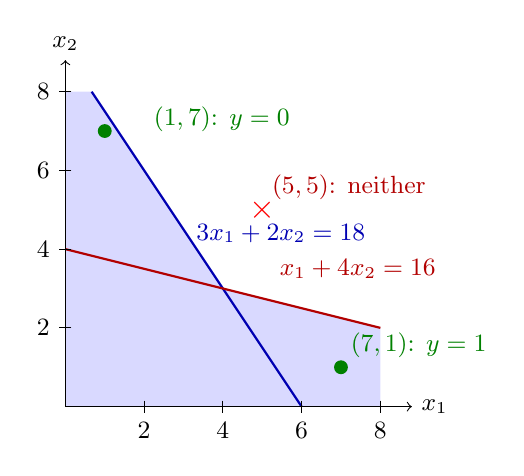
\begin{tikzpicture}[every node/.style={font=\small}, x=0.5cm, y=0.5cm]
	\fill[blue!15] (0,0) -- (6,0) -- (0.667,8) -- (0,8) -- cycle;
	\fill[blue!15] (0,0) -- (8,0) -- (8,2) -- (0,4) -- cycle;
	\draw[blue!70!black, thick] (0.667,8) -- (6,0) node[pos=0.45, right, font=\small] {$3x_1+2x_2=18$};
	\draw[red!70!black, thick] (0,4) -- (8,2);
	\node[red!70!black, font=\small, anchor=south west] at (5.2,3.0) {$x_1+4x_2=16$};
	\draw[->] (0,0) -- (8.8,0) node[right, font=\small] {$x_1$};
	\draw[->] (0,0) -- (0,8.8) node[above, font=\small] {$x_2$};
	\foreach \x in {2,4,6,8} {\draw (\x,0.15) -- (\x,-0.15) node[below, font=\small] {$\x$};}
	\foreach \y in {2,4,6,8} {\draw (0.15,\y) -- (-0.15,\y) node[left, font=\small] {$\y$};}
	\fill[green!50!black] (7,1) circle (2.5pt); \node[green!50!black, font=\small, above right] at (7,1) {$(7,1)$: $y=1$};
	\fill[green!50!black] (1,7) circle (2.5pt); \node[green!50!black, font=\small, anchor=west] at (2.0,7.3) {$(1,7)$: $y=0$};
	\node[red, font=\large] at (5,5) {$\times$}; \node[red!70!black, font=\small, above right] at (5,5) {$(5,5)$: neither};
	\end{tikzpicture}
\end{document}
